%! Author = guerster
%! Date = 13.11.21

\documentclass{beamer}

\usepackage[ngerman]{babel}
\usepackage{graphicx}
\usepackage{wasysym}
\usepackage{textcomp}
\usepackage{todonotes}


% Example here:
% https://github.com/josephwright/beamer/blob/main/doc/solutions/conference-talks/conference-ornate-20min.de.tex

\mode<presentation>
{
    \usetheme{Singapore}
%\usetheme{AnnArbor}
%\usecolortheme{beaver}
}

\title{Kolloquium Entwurf}
\subtitle{SEP WS 2021/2022}

%\titlegraphic{
\includegraphics[width=5cm]{../../docs/Pflichtenheft/graphics/LasEs-logo}}

\date{\small 16. November 2021}
\logo{
\includegraphics[width=1.5cm]{../../docs/Pflichtenheft/graphics/LasEs-logo}}

\author{\textbf{Team 2} \\ \small {Johannes Garstenauer, Stefanie Gürster, Thomas Kirz,\\ Johann Schicho, Sebastian Vogt} \\ \vspace{0.5cm}\emph{Phasenleiter: Stefanie Gürster}\normalsize}


\begin{document}

    \begin{frame}
        \titlepage
    \end{frame}

    \begin{frame}{Gliederung}
        \tableofcontents
    \end{frame}


    \section{Architektur}

    \begin{frame}{Schichtenarchitektur}
        \begin{itemize}

            \item Aufteilung in vier Schichten \pause
            \item Model View Controller
            \pause
            \begin{itemize}
                \item View
                \item Control
                \item Business
                \item Persistence
            \end{itemize}

        \end{itemize}
    \end{frame}

    \begin{frame}{Paketstruktur}
        \centering
        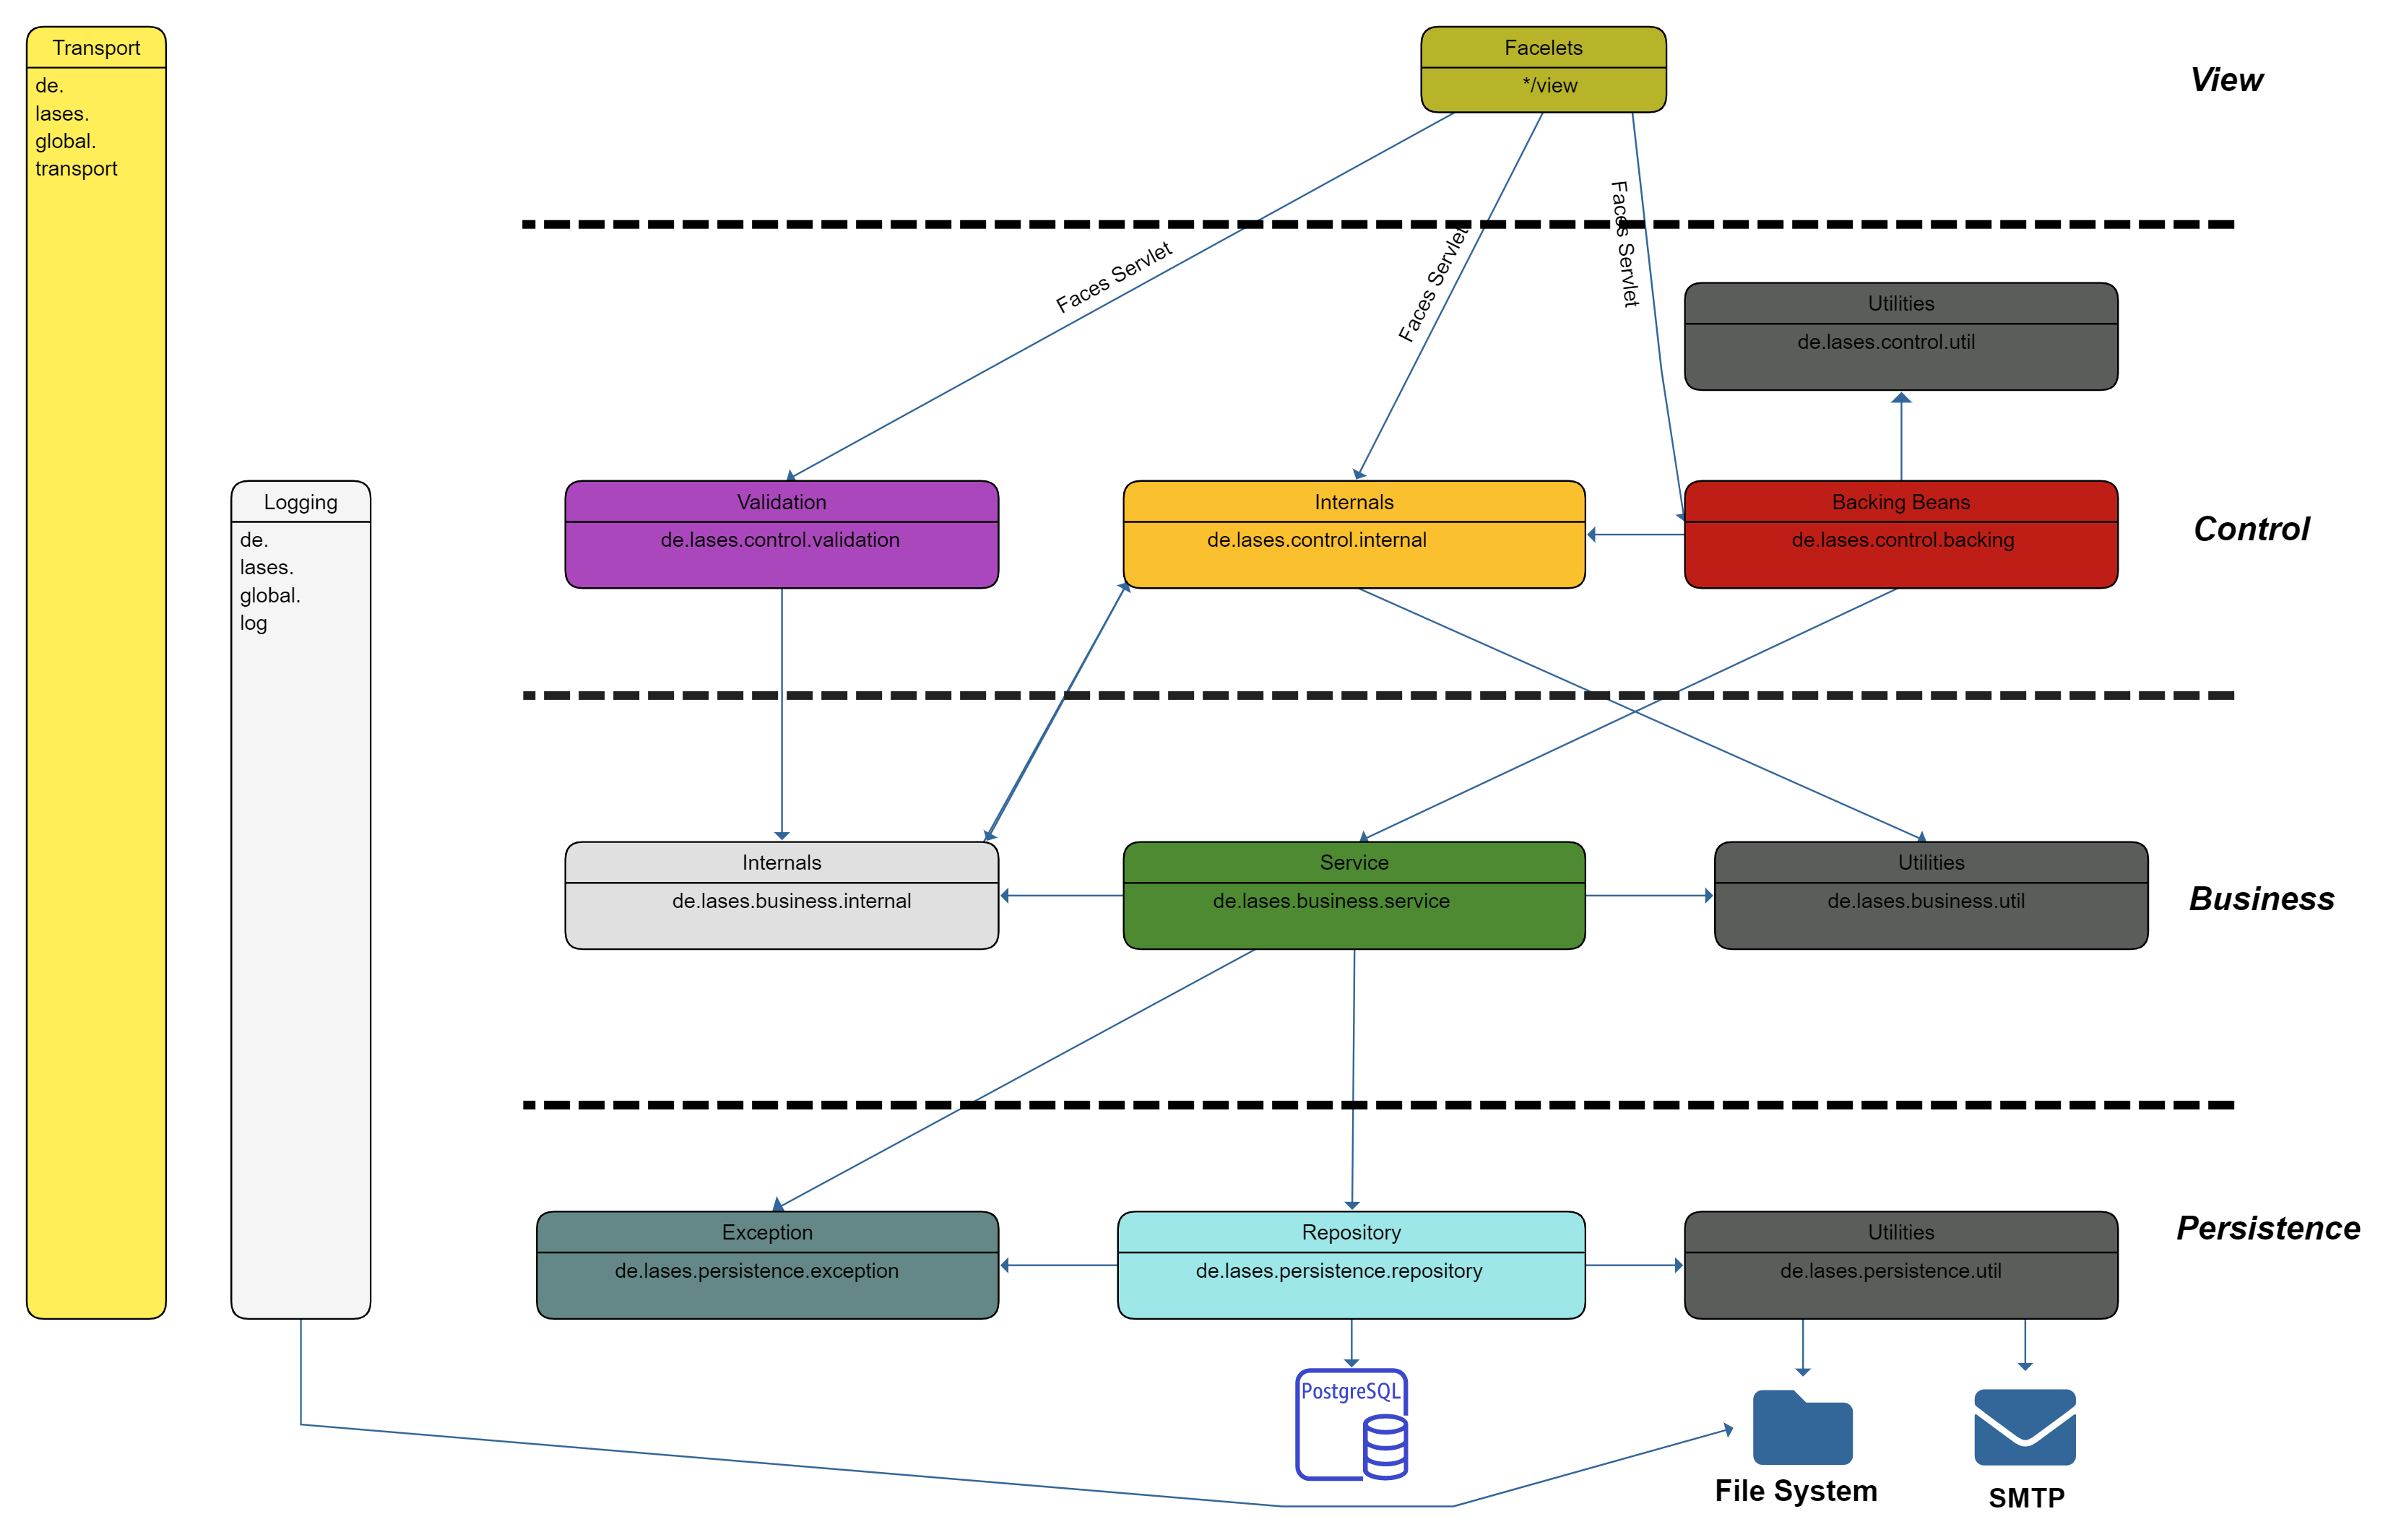
\includegraphics[width=0.9\textwidth]{../../docs/Entwurf/graphics/Paketdiagramm9.0.png}
    \end{frame}

    \begin{frame}{Klassendiagramm}
        \centering
        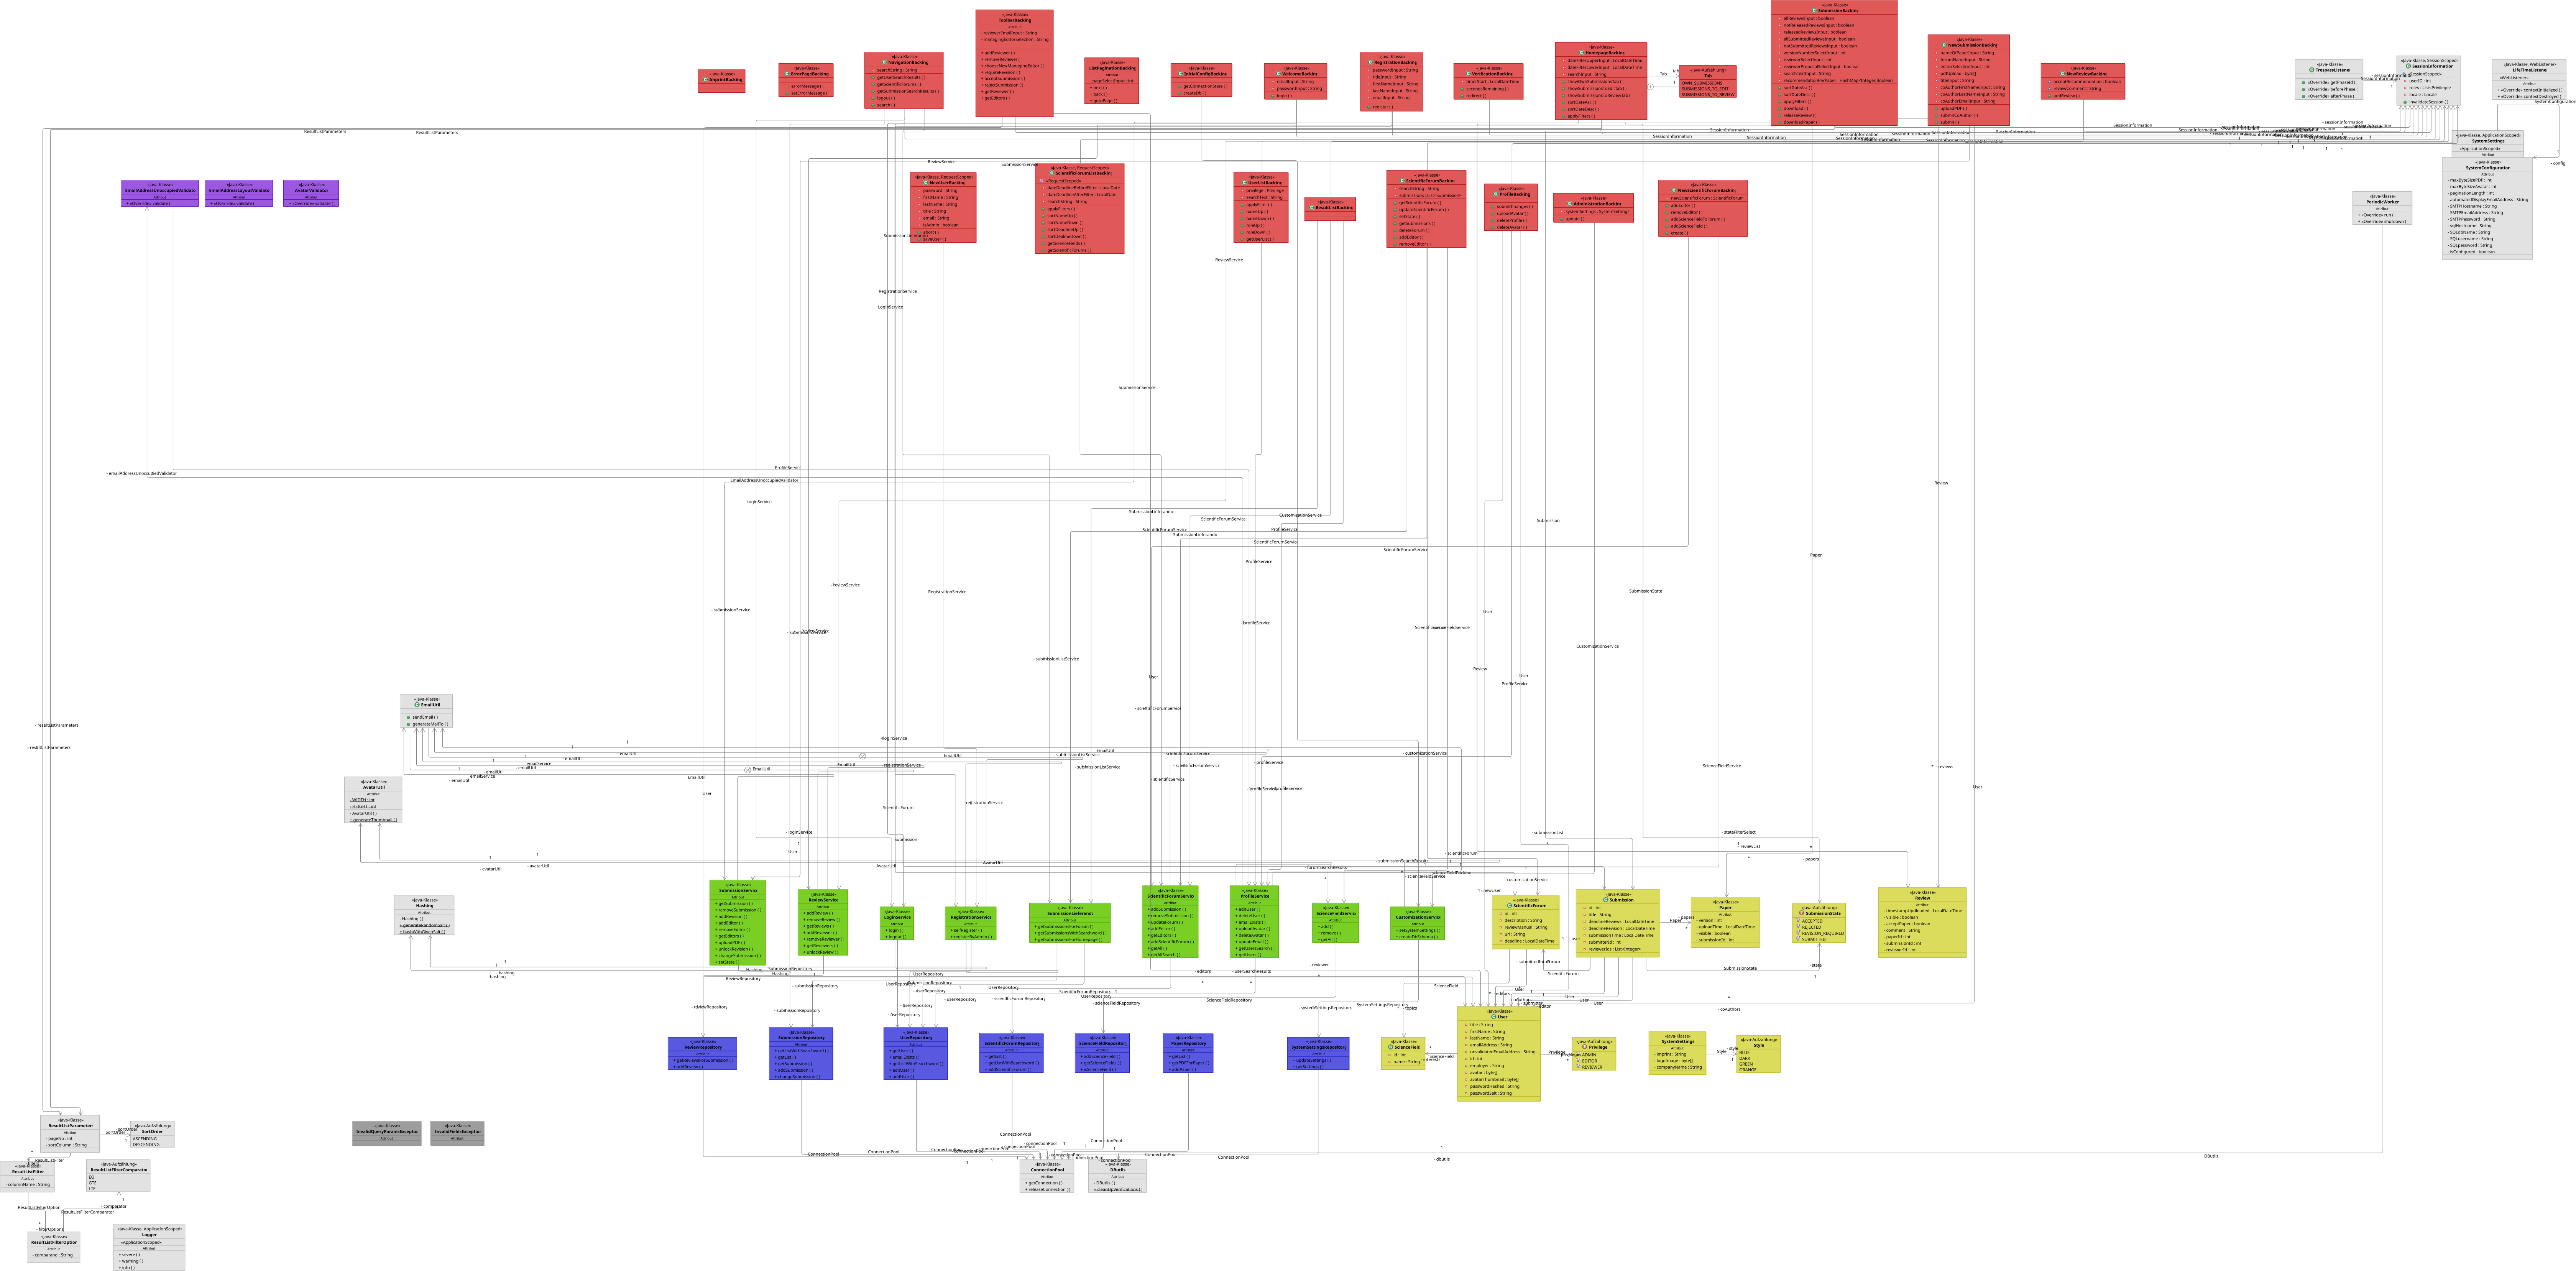
\includegraphics[width=0.9\textwidth]{../../docs/Entwurf/graphics/klassendiagramm_png.png}
    \end{frame}



    \section{Szenario}
    \begin{frame}{Aufruf einer Submission}
        \centering
        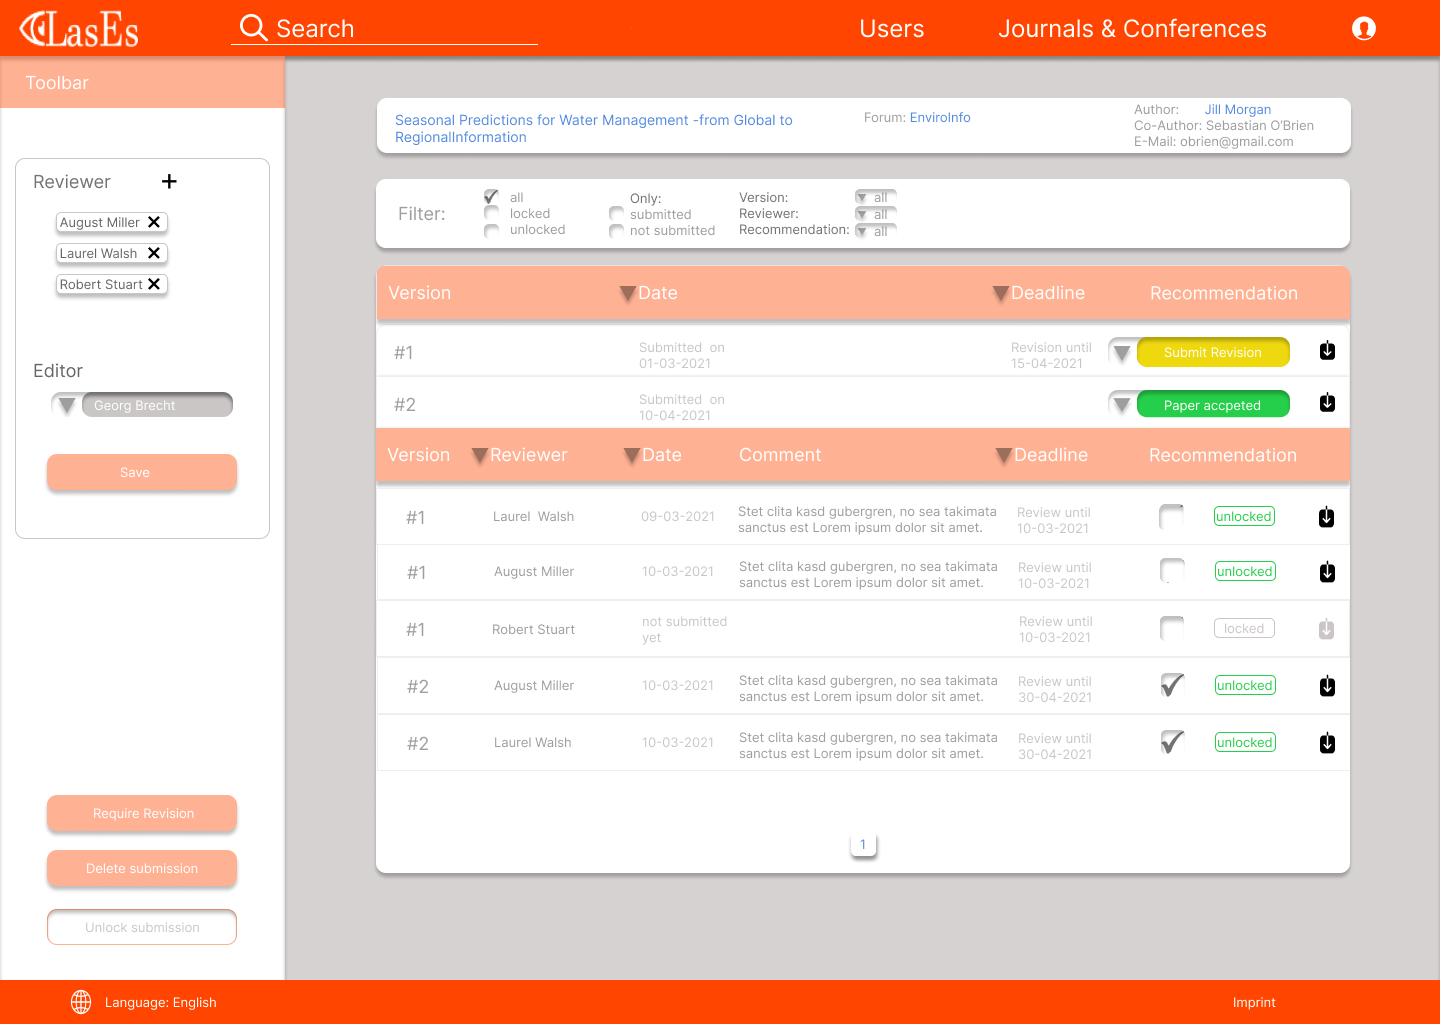
\includegraphics[width=\textwidth]{../../docs/Pflichtenheft/graphics/Submission-png.png}
    \end{frame}

    \begin{frame}{Sequenzdiagramm}
        \centering
        Sequenzdaigramm 1
    \end{frame}

    \begin{frame}{control.backing}
        \centering
        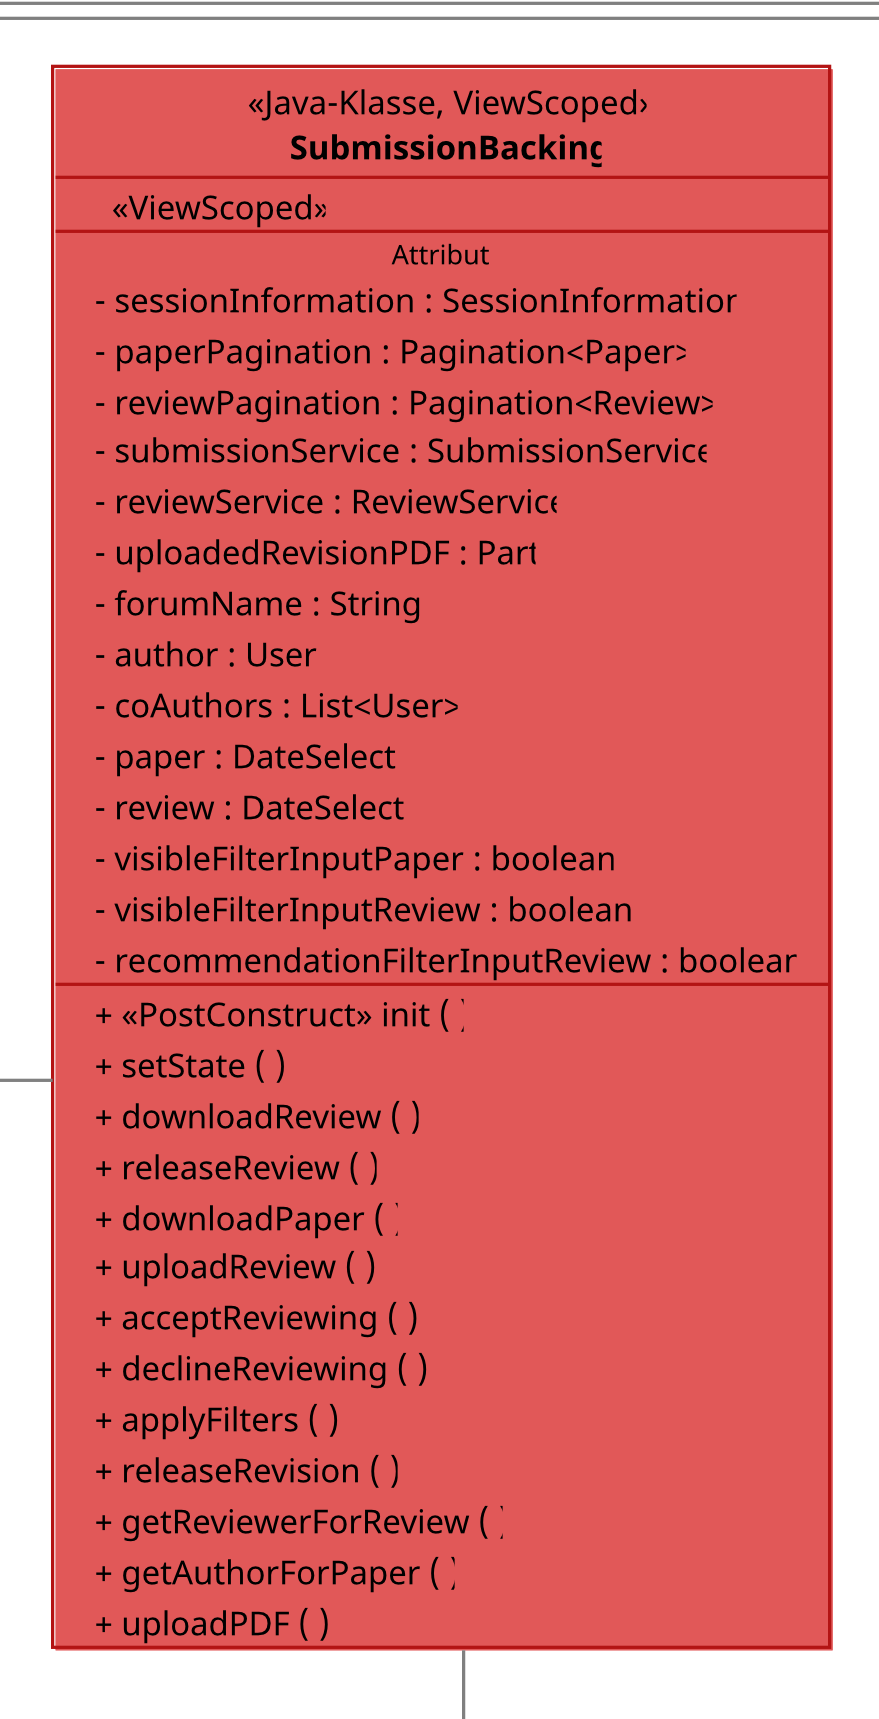
\includegraphics[height=0.9\textheight]{excerpts/SubmissionBacking@3x}
    \end{frame}

    \begin{frame}{global.transport}
        \centering
        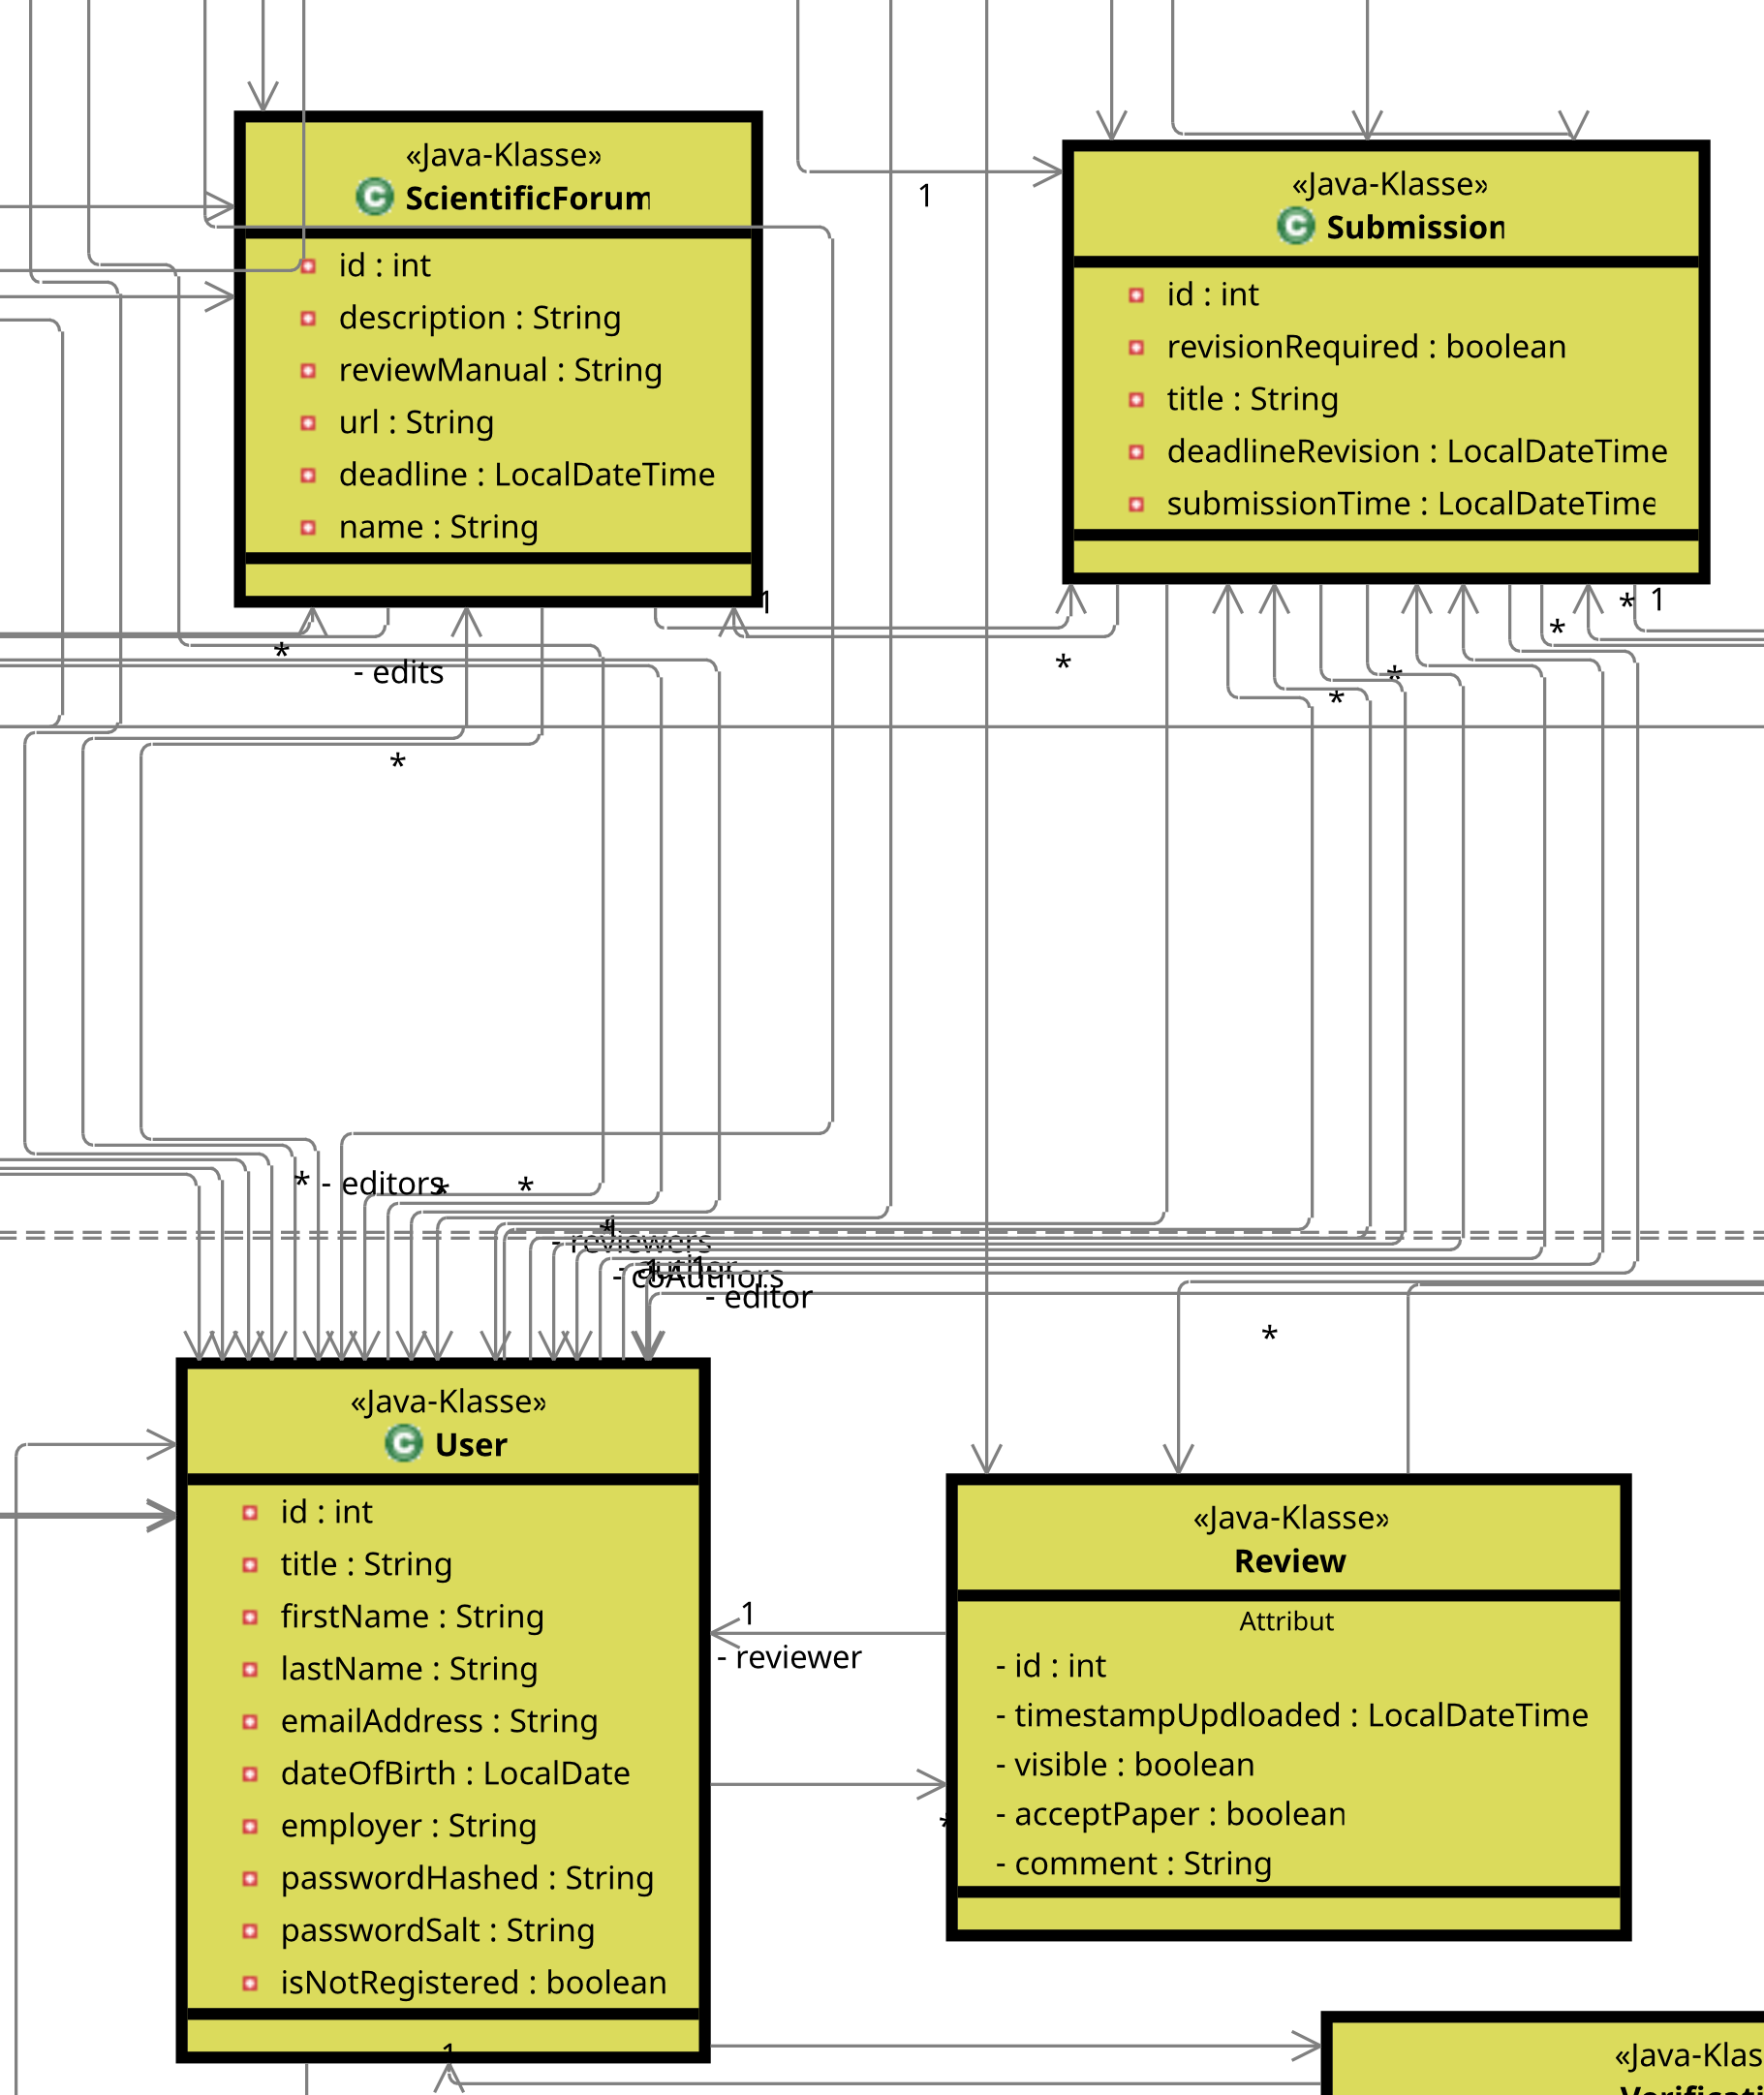
\includegraphics[height=0.9\textheight]{excerpts/Submission+User@3x}
    \end{frame}

    \begin{frame}{business.service}
        \centering
        SubmissionService
    \end{frame}

    \section{Rechteprüfung}

    \begin{frame}{Rechteprüfung}
        \begin{itemize}
            \item Trespasslistener \pause
            \item Schaltflächen abhängig von Nutzerrollen \pause
            \item Exception
        \end{itemize}
    \end{frame}

    \begin{frame}{Sequenzdiagramm}
        \centering
        Sequenzdiagramm 2
    \end{frame}

    \section{Szenario}
    \begin{frame}{persistence.repository}
        \centering
        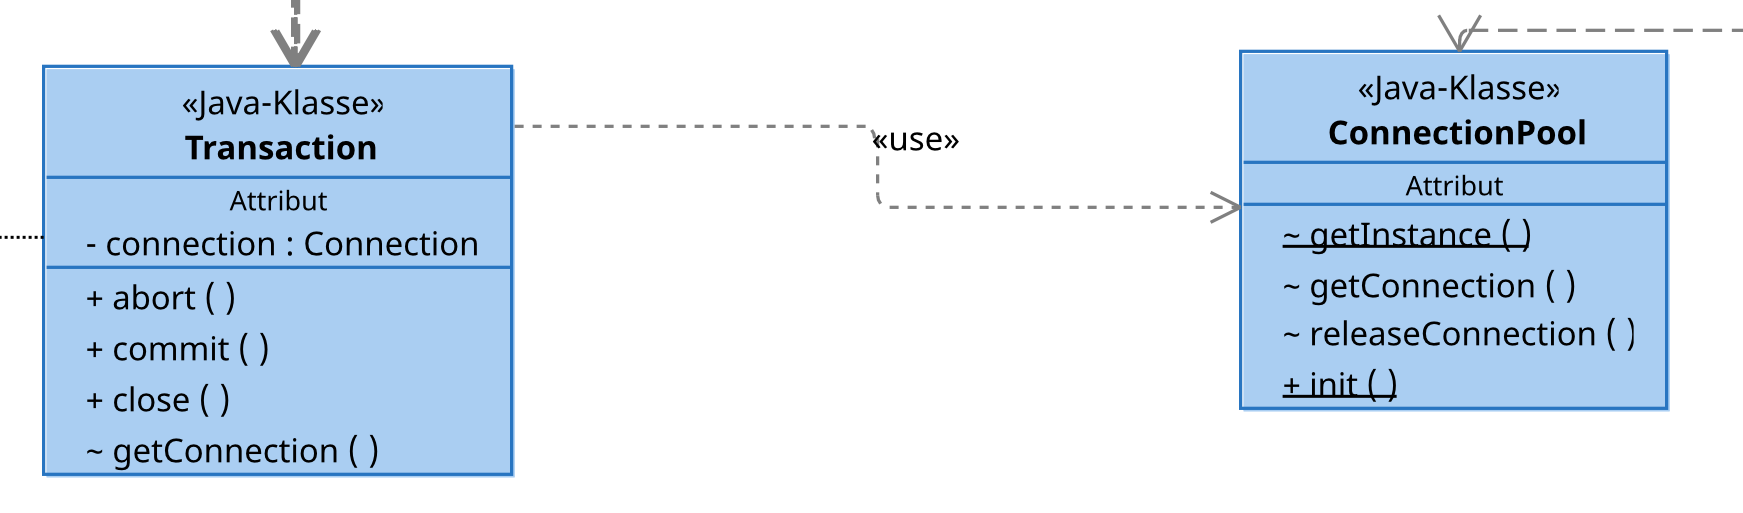
\includegraphics[width=\textwidth]{excerpts/Transaction+ConnectionPool@3x}
    \end{frame}

    \begin{frame}{persistence.repository}
        \centering
        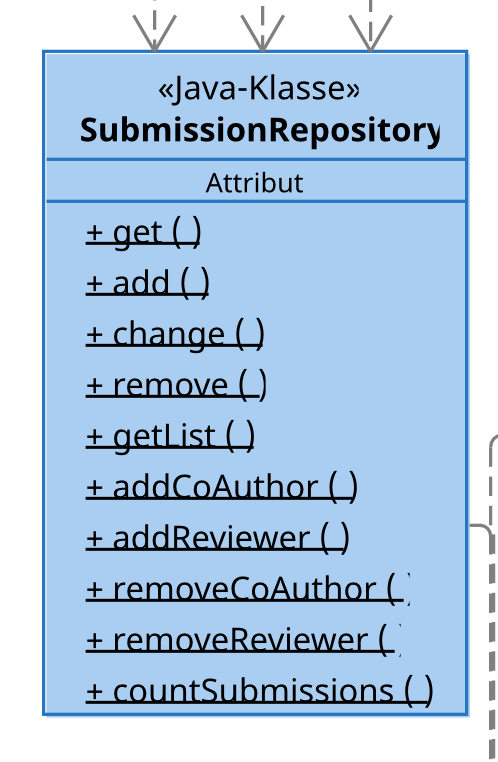
\includegraphics[height=0.9\textheight]{excerpts/SubmissionRepository@3x}
    \end{frame}

    \begin{frame}{ER-Diagramm}
        \centering
        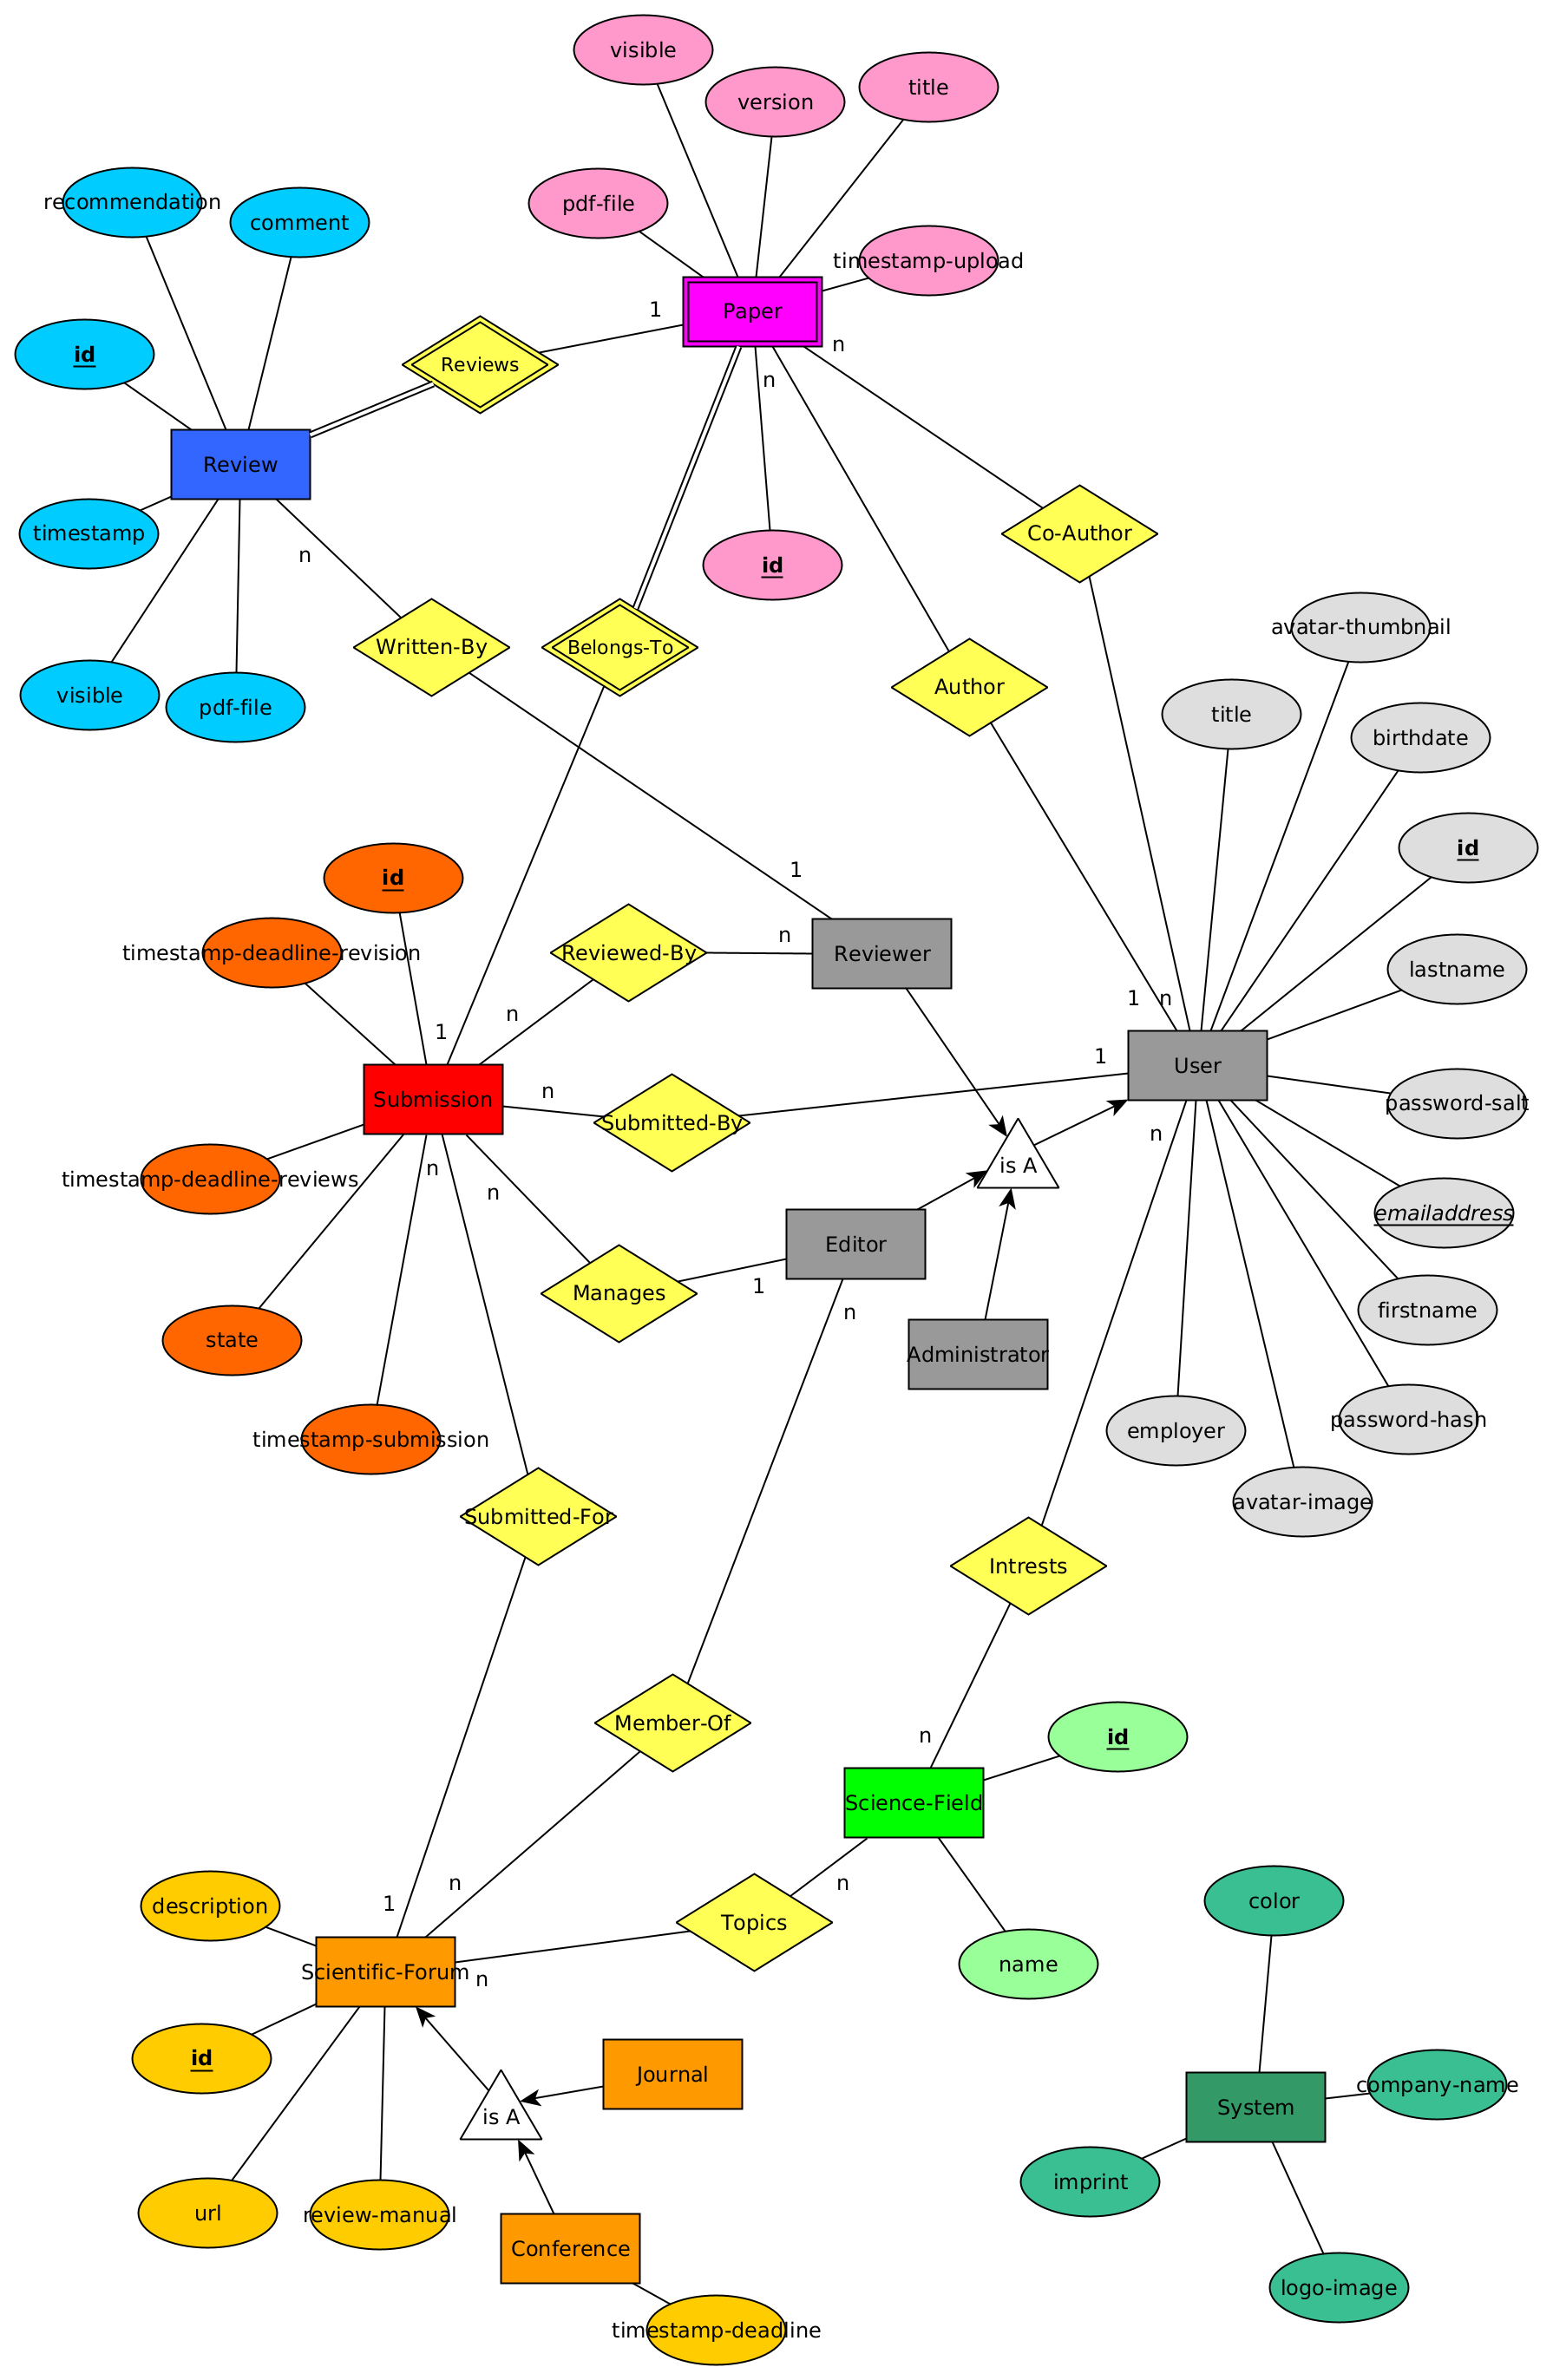
\includegraphics[height=0.9\textheight]{../../docs/Entwurf/graphics/ER-Modell.png}
    \end{frame}

    \begin{frame}{Sequenzdiagramm}
        \centering
        Sequenzdiagramm 3
    \end{frame}

    \begin{frame}{Facelet}
        \begin{itemize}
            \item Templates
            \item Content
            \item Composite Components
        \end{itemize}
    \end{frame}

%    \begin{frame}{Abstraktion}
%        \begin{itemize}
%            \item Transaction Objects
%            \item Repositories
%        \end{itemize}
%    \end{frame}
%
%    \begin{frame}{Schwache Kopplung}
%        \begin{itemize}
%            \item MVC-Pattern \pause
%            \item Persistenzschicht
%        \end{itemize}
%        Technologien werden austauschbar.
%    \end{frame}
%
%    \begin{frame}{Hohe Kohäsion}
%        \begin{itemize}
%            \item Jeder Service hat eine Aufgabe
%            \pause
%            \item Jedes Repository kümmert sich um ein DTO
%            \pause
%            \item Jedes Backing Bean hat ein Facelet \pause
%            \item Ein DTO speichert Daten von genau einer Entität
%        \end{itemize}
%    \end{frame}
%
%    \begin{frame}{Lokalisierung}
%        \begin{itemize}
%            \item Internationalisierung
%        \end{itemize}
%    \end{frame}
%
%    \begin{frame}{Demeter Prinzip}
%        \begin{itemize}
%            \item Kommunikation nur mit eigener oder angrenzender Schicht
%        \end{itemize}
%    \end{frame}


    \section{Fehlerbehandlung}

    \begin{frame}{Geprüfte Ausnahmen}
        \pause
        \begin{columns}
            \begin{column}{.48\textwidth}
                Persistenz Schicht
                \begin{itemize}
                    \item Kapselung in semantisch passende Ausnahmeklassen
                \end{itemize}
            \end{column}
            \pause
            \begin{column}{.48\textwidth}
                Business- und Kontrollschicht
                \begin{itemize}
                    \item Auslösen eines Events
                    \item Fangen durch UIGenerator
                \end{itemize}
            \end{column}
        \end{columns}
    \end{frame}

    \begin{frame}{Ungeprüfte Ausnahmen}
        \begin{itemize}
            \item UncheckedExceptionHandler
        \end{itemize}
    \end{frame}

    \begin{frame}{Sequenzdiagramm}
        \centering
        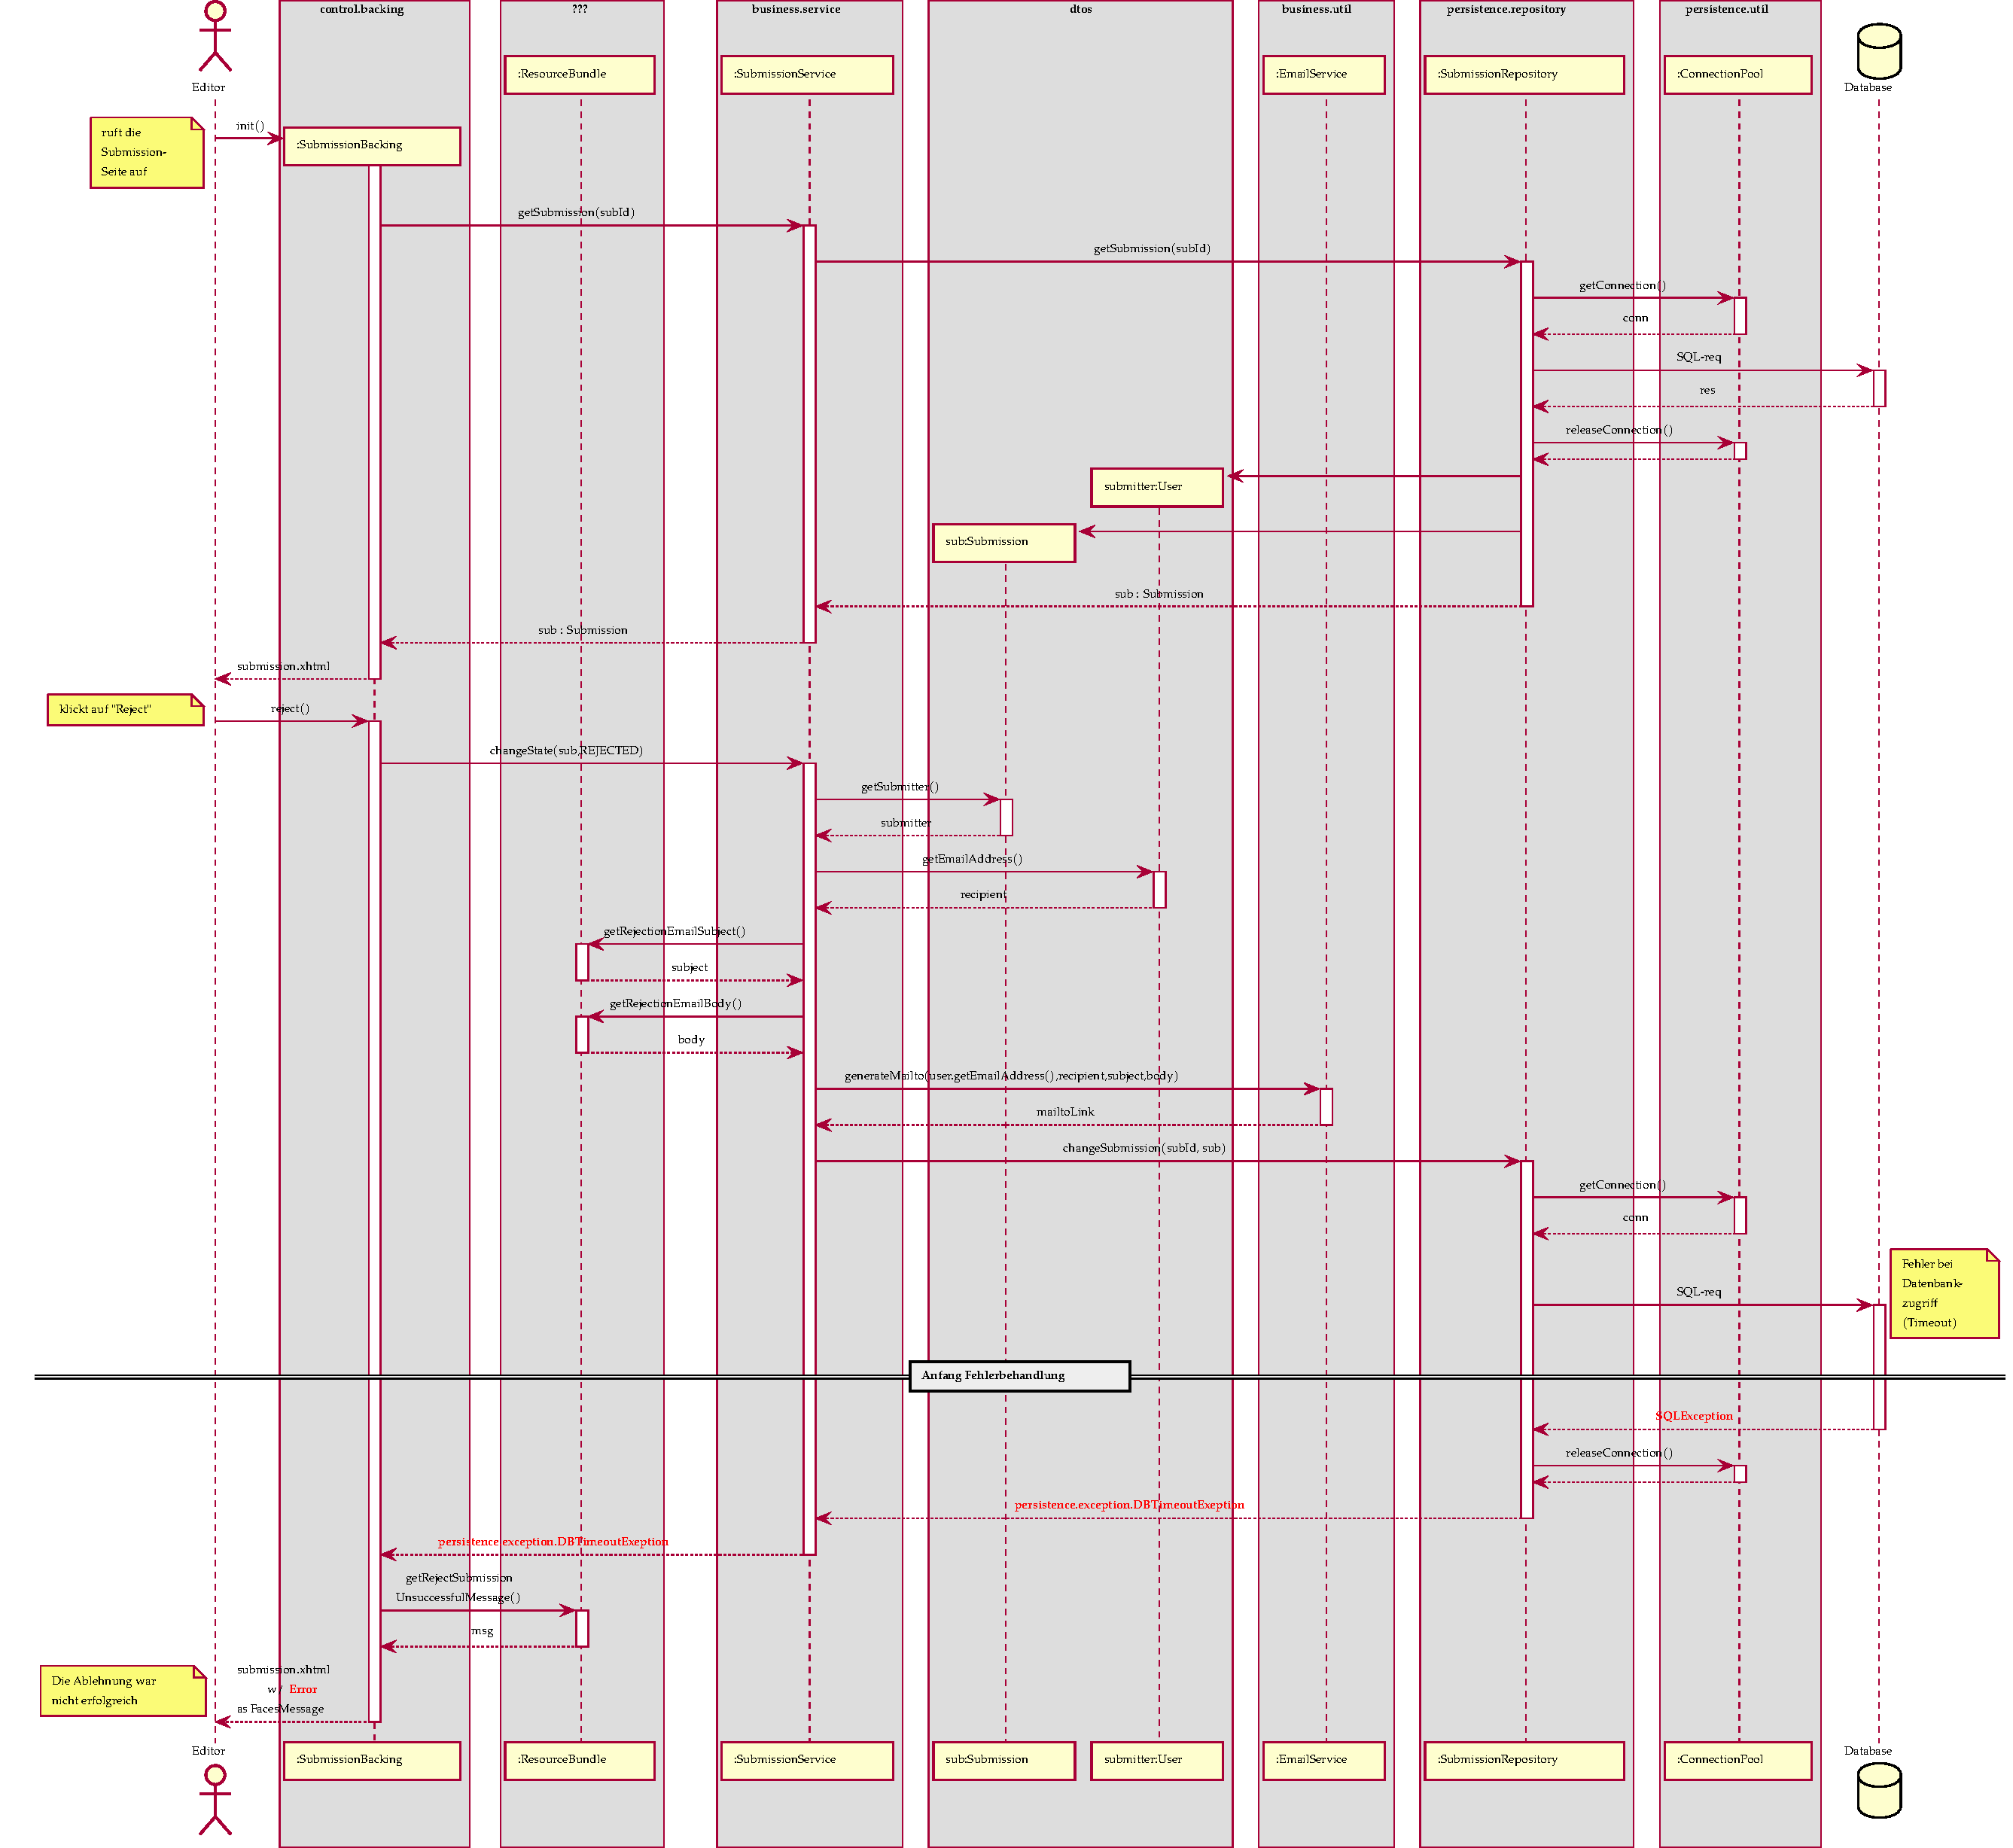
\includegraphics[height=0.9\textheight]{../../docs/Entwurf/graphics/reject_submission.pdf}
    \end{frame}
    

    \section{Prinzipien}

    \begin{frame}{Prinzipien}
        \begin{itemize}
            \item Abstraktion \pause
            \item Schwache Kopplung \pause
            \item Hohe Kohäsion \pause
            \item Lokalisierung \pause
            \item Demeter Prinzip
        \end{itemize}
    \end{frame}


    \section{Konventionen}
    \begin{frame}{Konventionen}
        \pause
        \begin{itemize}
            \item Zuordnung durch ID's
            \item x \textrightarrow 1
            \item x \textrightarrow * \pause
            \item Jedes Backing Bean genau ein Facelet \pause
            \item Methoden \emph{getList()} und \emph{change()}
        \end{itemize}
    \end{frame}



    \section{Evolution}
    \begin{frame}{Evolutionsfähigkeit}
        \begin{itemize}
            \item Schichtenarchitektur
            \item Internationalisierung
            \item Einfache Erweiterung
        \end{itemize}
    \end{frame}

    \section{Diskussion}
    \begin{frame}{Diskussion}
        
\includegraphics[width=\textwidth]{../../docs/Pflichtenheft/graphics/LasEs-logo}
    \end{frame}

\end{document}
